\clearpage

\section{Photoelectron Generator}

\begin{tcolorbox}	
\begin{tabular}{p{2.75cm} p{0.2cm} p{10.5cm}} 	
\textbf{Header File}   &:& photoelectron\_generator\_*.h \\
\textbf{Source File}   &:& photoelectron\_generator\_*.cpp \\
\textbf{Version}       &:& 20180302 (Diamantino Silva)
\end{tabular}
\end{tcolorbox}

\vspace{1em}

This block simulates the generation of photoelectrons by a photodiode, performing the conversion of an incident electric field into an output current proportional to the field's instantaneous power.
It is also capable of simulating shot noise.
%
\begin{figure}[h]
	\centering
	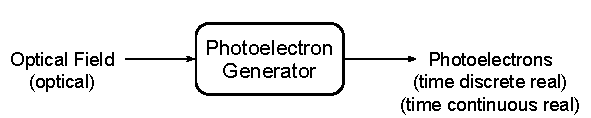
\includegraphics{./lib/photoelectron_generator/figures/photoelectron_generator_scheme.pdf}
	\caption{Schematic representation of the photoelectron generator code block}
\end{figure}

\subsection*{Theoretical description}

The operation of a real photodiode is based on the photoelectric effect, which consists on the removal of one electron from the target material by a single photon, with a probability $\eta$.
Given an input beam with an optical power $P(t)$ in which the photons are around the wavelength $\lambda$, the flux of photons $\phi(t)$ is calculated as
\cite{saleh1991}
%
\begin{equation}
	\phi(t) = \frac{P(t) \lambda}{hc}
\end{equation}
therefore, the mean number of photons in a given interval $\left[ t, t+T \right[$ is
\begin{equation}
	\bar{n}(t) = \int_{t}^{t+T} \phi(\tau) \; \textrm{d}\tau
\end{equation}
%
But the actual number of photons in a given time interval, $n(t)$, is random. If we assume that the electric field is generated by an ideal laser with constant power, then $n(t)$ will follow a Poisson distribution
%
\begin{equation}
	p\left( n \right) = \frac{ \bar{n}^n \exp(-\bar{n})}{n!}
\end{equation}
%
where $n=n(t)$ and $\bar{n} = \bar{n}(t)$.
\\
For each incident photon, there is a probability $\eta$ of generating a phototelectron.
Therefore, we can model the generation of photoelectrons during this time interval, as a binomial process where the number of events is equal to the number of incident photons, $n(t)$, and the rate of success is $\eta$.
If we combine the two random processes, binomial photoelectron generation after poissonian photon flux, the number of output photoelectrons in this time interval, $m(t)$, will follow
\cite{saleh1991}
%
\begin{equation}
	m \sim \textrm{Poisson}\left(\eta \bar{n} \right)
	\label{eq:electron_number_distribution}
\end{equation}
%
with $\bar{m} = \eta \bar{n}$ where $m = m(t)$.
%
%
%
%
\subsection*{Functional description}
%
The input of this block is the electric field amplitude, $A(t)$, with sampling period $T$.
The first step consists on the calculation the instantaneous power.
Given that the input amplitude is a baseband representation of the original signal, then $P(t) = 4 |A(t)|^2$.
From this result, the average number of photons $\bar{n}(t) = T P(t) \lambda / h c$.\\
If the shot-noise is negleted, then the output number of photoelectrons, $n_e(t)$ in the interval, will be equal to
%
\begin{equation}
	m(t) = \eta \overline{n(t)}
\end{equation}
%
If the shot-noise is considered, then the output fluctuations will be simulated by generating a value from a Poissonian random number generator with mean $\eta \overline{n(t)}$
\begin{equation}
	m(t) \sim \textrm{Poisson}\left(\eta \overline{n(t)} \right)
\end{equation}

\subsection*{Input Parameters}

\begin{table}[H]
	\centering
	\label{my-label}
	\begin{tabular}{|c|c|c|}
		\hline
		\textbf{Parameter}	& \textbf{Default Value}	& \textbf{Description} \\
		\hline
		efficiency			& 1.0						& Photodiode's quantum efficiency. \\
		\hline
		shotNoise			& false 					& Shot-noise off/on. \\
		\hline
	\end{tabular}
\end{table}




\subsection*{Methods}

PhotoelectronGenerator()
\bigbreak
PhotoelectronGenerator(vector$<$Signal *$>$ \&InputSig, vector$<$Signal *$>$ \&OutputSig) :Block(InputSig, OutputSig) {}
\bigbreak
void initialize(void)
\bigbreak
bool runBlock(void)
\bigbreak
void setEfficiency(\texttt{t\_real} efficiency)
\bigbreak
void getEfficiency()
\bigbreak
void setShotNoise(\texttt{bool} shotNoise)
\bigbreak
void getShotNoise()
%
%
%
%
\pagebreak

\subsection*{Input Signals}

\subparagraph*{Number:} 1

\subparagraph*{Type:} Optical (OpticalSignal)

\subsection*{Output Signals}

\subparagraph*{Number:} 1

\subparagraph*{Type:} Electrical (TimeDiscreteAmplitudeContinuousReal or TimeContinuousAmplitudeContinuousReal)

\subsection*{Examples}

\begin{figure}[h]
	\centering
	
\includegraphics{./lib/photoelectron_generator/figures/scheme_simulation_constant.pdf}
	\caption{Constant power simulation setup}
\end{figure}

To test the output of this block, we recreated the results of figure $11.2-3$ in \cite{saleh1991}.
We started by simulating the constant optical power case, in which the local oscillator power was fixed to a constant value.
Two power levels were tested, $P = 1 \mu W$ and $P = 1 nW$, using a sample period of $20$ picoseconds and photoelectron generator efficiency of $1.0$.
The simulation code is in folder \texttt{lib \textbackslash photoelectron\_generator \textbackslash photoelectron\_generator\_test\_constant}.
The following plots show the number of output electrons per sample when the shot noise is ignored or considered

\begin{figure}[H]
	\centering
	\begin{subfigure}{0.45\textwidth}
		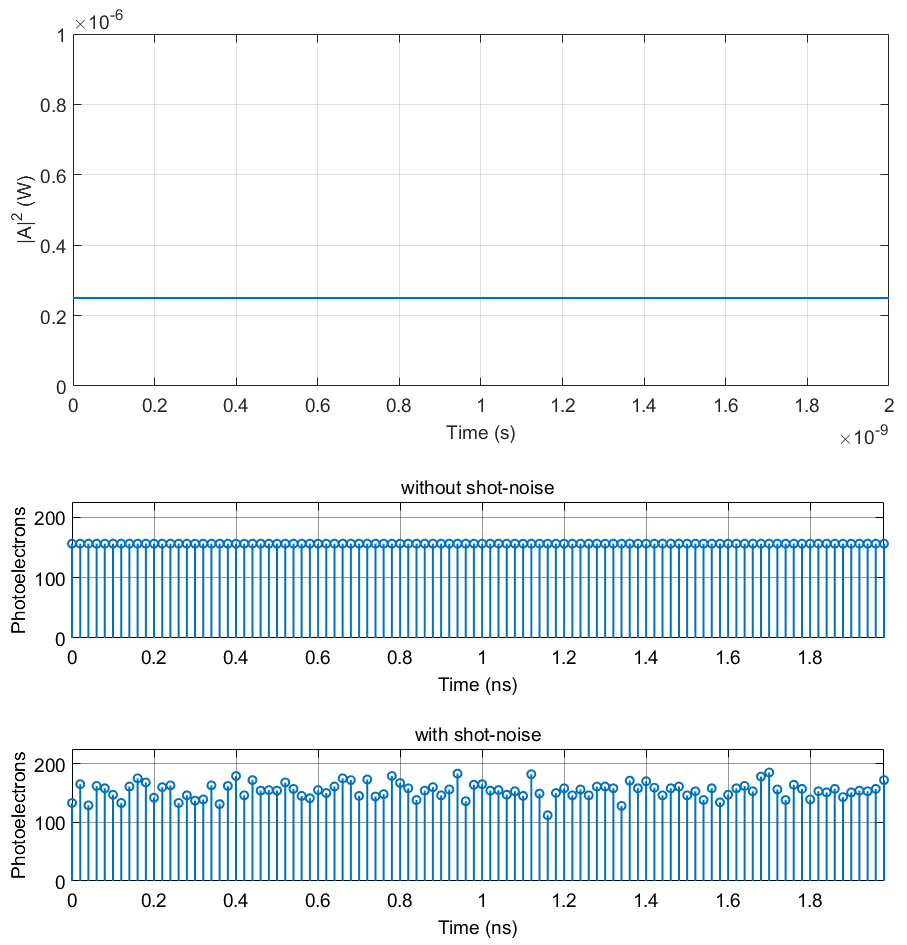
\includegraphics[width=\textwidth]{./lib/photoelectron_generator/figures/plot-constant-1uW}
		\caption{$P=1 \mu W$}
	\end{subfigure}
	\hspace{10mm}
	\begin{subfigure}{0.45\textwidth}
		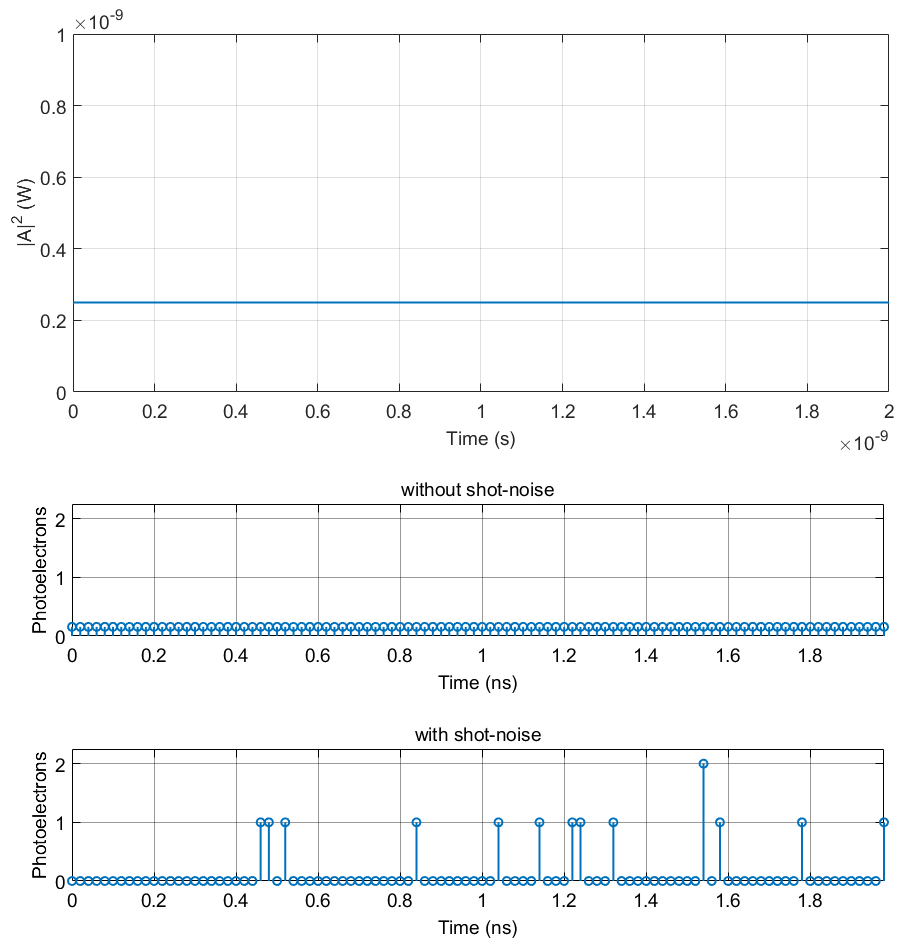
\includegraphics[width=\textwidth]{./lib/photoelectron_generator/figures/plot-constant-1nW}
		\caption{$P=1 nW$}
	\end{subfigure}
	\caption{Upper plots: input optical squared amplitude on the photoelectron generator; Middle plots: number of output photoelectrons per sample neglecting quantum noise; Bottom plots: number of output photoelectrons per sample considering quantum noise.}
	\label{plot:quantum_noise_sim_constant}
\end{figure}
%
Figure \ref{plot:quantum_noise_sim_constant} shows clearly that turning the quantum noise on or off will produce a signal with or without variance, as predicted.
If we compare this result with plot $(a)$ in \cite{saleh1991}, in particular $P=1nW$, we see that they are in conformance, with a slight difference, where a sample has more than one photoelectron.
In constrast with the reference result, where only single events are represented, the $P=1 \mu W$ case shows that all samples account many photoelectrons.
Given it's input power, multiple photoelectron generation events will occur during the sample time window.
Therefore, to recreate the reference result, we just need to reduce the sample period until the probability of generating more than $1$ photoelectron per sample goes to $0$.
\\
%
\begin{figure}[H]
	\centering
	
\includegraphics{./lib/photoelectron_generator/figures/scheme_simulation_variable.pdf}
	\caption{Variable power simulation setup}
\end{figure}
%
To recreate plot $(b)$ in \cite{saleh1991}, a more complex setup was used, where a series of states are generated and shaped by a MQAM, creating a input electric field with time-varying power.\\
The simulation code is in folder \texttt{lib \textbackslash photoelectron\_generator \textbackslash photoelectron\_generator\_test\_variable}.
%
\begin{figure}[H]
	\centering
	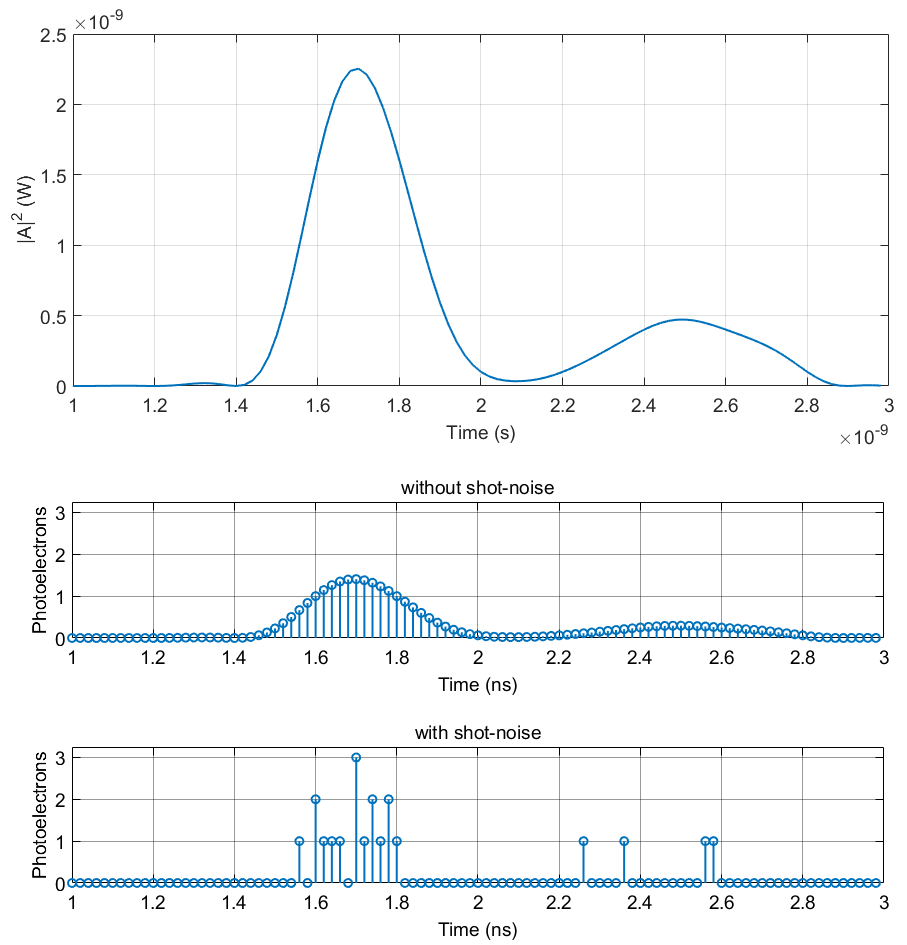
\includegraphics[width=0.45\textwidth]{./lib/photoelectron_generator/figures/plot-variable}
	\caption{Upper plots: input optical squared amplitude on the photoelectron generator; Middle plots: number of output photoelectrons per sample neglecting quantum noise; Bottom plots: number of output photoelectrons per sample considering quantum noise.}
	\label{plot:quantum_noise_sim_variable}
\end{figure}
%
Figure \ref{plot:quantum_noise_sim_variable} shows that the output without shot-noise is following the input power perfectly, apart from a constant factor. In the case with shot-noise, we see a that there are only output samples in high power input samples.\\
These results are not following strictly plot $(b)$ in \cite{saleh1991}, because has already discussed previously, in the high power input samples, we have a great probability of generating many photoelectrons.
%
\subsection*{Sugestions for future improvement}

%\bibliography{./lib/photoelectron_generator/photoelectron_generator}
